
\documentclass[notheorems,hyperref={pdfpagelabels=true},xcolor={table}]{beamer}
%\setlength{\textwidth}{0.7\paperwidth}

\usepackage{amsmath}
\usepackage{amssymb}

\usetheme{minflat}

\usepackage{booktabs}
\usepackage[scale=2]{ccicons}
\usepackage{verbatim}

\usepackage[style=american]{csquotes}
\usepackage{tikz}
\usepackage{graphicx}
\usepackage[export]{adjustbox}



\usetikzlibrary{decorations.pathreplacing, decorations.pathmorphing,calc,arrows,positioning}

%%% enable notes on second screen
%\usepackage{pgfpages}
%\setbeameroption{show notes on second screen=right}
%\setbeamertemplate{note page}[compress]

	
%%%%%%%%%%%%%%%%%%%%%%%%%%%%%%%%%%%%%%%%%%%%%%%%%%%
%%%%	define content of title page
%%%%%%%%%%%%%%%%%%%%%%%%%%%%%%%%%%%%%%%%%%%%%%%%%%%
\def\talkTitle{Sample/feature-based explanations for AI Solution}
\def\talkShortTitle{Data-based XAI}
\def\talkSubtitle{Empirical Systems Engineering and Modeling}
\def\talkKeywords{}

%% Define meta data of pdf
\hypersetup{
    pdftitle={Slides to talk - \talkTitle},
	pdfsubject={\talkTitle},
	pdfauthor={Levente Alekszejenkó},
	pdfkeywords={\talkKeywords},
	colorlinks=false
}


\newcommand\blurredimagetotal[1]{
	\node[opacity=0.1, anchor=west, inner sep=0pt] (left) at (current page.west) {\adjincludegraphics[width = \paperwidth, height=\paperheight]{#1}};
}

\newcommand\blurredimagesimple[2]{
	\node[opacity=0.1, anchor=west, inner sep=0pt] (left) at (current page.west) {\adjincludegraphics[width = 0.8\paperwidth, height=\paperheight, trim={0, 0, 0.2\width, 0}, clip]{#2}};
	
	\node[anchor=east, inner sep=0pt] at (current page.east){\adjincludegraphics[width = 0.2\paperwidth, height=\paperheight, trim={0.8\width, 0, 0, 0}, clip]{#1}};
}

\newcommand\blurredframe[2]{
		\begin{center}
			\begin{tikzpicture}[remember picture, overlay]
			\blurredimagesimple{#1}{#2}
			\end{tikzpicture}
		\end{center}
}

\newcommand\blurredtotalframe[1]{
	\begin{center}
		\begin{tikzpicture}[remember picture, overlay]
		\blurredimagetotal{#1}
		\end{tikzpicture}
	\end{center}
}


%%%%%%%%%%%%%%%%%%%%%%%%%%%%%%%%%%%%%%%%%%%%%%%%%%%
%%%%	set content of title page
%%%%%%%%%%%%%%%%%%%%%%%%%%%%%%%%%%%%%%%%%%%%%%%%%%%
\title[\talkShortTitle]{\talkTitle}  
\subtitle{\talkSubtitle} 
\author{{Alekszejenkó Levente -- alelevente@mit.bme.hu}}
%\DTMlangsetup[hu-HU]{ord=raise,monthyearsep={.\space}}
%\date{\DTMtoday}
\date{2022. december 1.}
\institute{%
	
\includegraphics[width=\textwidth]{./gfx/bme_mit.png}%
}

%%%%%%%%%%%%%%%%%%%%%%%%%%%%%%%%%%%%%%%%%%%%%%%%%%%
%%%%	theorem tools, theorem and proof styles
%%%%%%%%%%%%%%%%%%%%%%%%%%%%%%%%%%%%%%%%%%%%%%%%%%%
\setbeamertemplate{theorem}[ams style]
%\setbeamertemplate{theorems}[numbered]

\newcounter{chapter}
\setcounter{chapter}{1}
\theoremstyle{plain}
\newtheorem{theorem}{Theorem}[section]
\newtheorem{lemma}[theorem]{Lemma}
\newtheorem{proposition}[theorem]{Proposition}
\newtheorem{corollary}[theorem]{Corollary}

\theoremstyle{definition}
\newtheorem{conclusion}[theorem]{Conclusion}
\newtheorem*{definition}{Definition}
\newtheorem*{remark}{Remark}
\newtheorem*{dummyblock}{dummyblock}

\theoremstyle{example}
\newtheorem{example}[theorem]{Example}

\newenvironment<>{dummyblock}[1]{%
	\setbeamercolor{block title}{fg=white,bg=white}%
	\setbeamercolor{block body}{fg=normal text.fg,bg=white}%
	\begin{block}#2{#1}\end{block}}

\setbeamerfont{section title}{size=\Huge,series=\bfseries}



\begin{document}

\renewcommand{\leq}{\leqslant}
\renewcommand{\geq}{\geqslant}

\renewcommand\theta\vartheta


%%%%%%%%%%%%%%%%%%%%%%%%%%%%%%%%%%%%%%%%%%%%%%%%%%%
%%%%	title page
%%%%%%%%%%%%%%%%%%%%%%%%%%%%%%%%%%%%%%%%%%%%%%%%%%%
\begin{frame}[plain]
	\titlepage
\end{frame}

\begin{frame}{In this lecture...}
    We will see two methods to explain AI classifier predictions.
    \vfill
    
    \begin{enumerate}
        \item Geometrical overview
        \item ProtoDash
        \item LIME
        \item Demo
    \end{enumerate}
    
    \vfill
    \textbf{Optimal training:} If multiple (complex enough) models were trained on an identical set of data, they cannot be distinguished by their prediction qualities.
\end{frame}

\begin{frame}{On the map of explainable AI}

    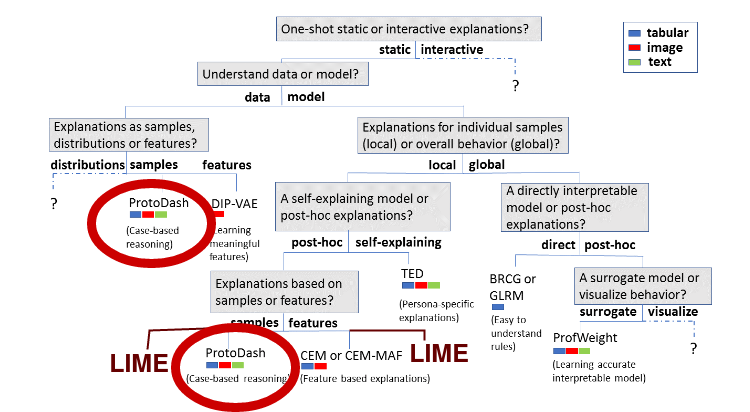
\includegraphics[width=\textwidth]{gfx/AIX-Page-4.drawio.png}
    \vfill
    Source: Arya et al., ``One Explanation Does Not Fit All: A Toolkit and Taxonomy of AI Explainability Techniques'', arXiv:1909.03012, 2019.
\end{frame}

\section[Geometry]{Geometrical interpretion}


\begin{frame}{A tabular representation}
    \begin{table}[]
        \centering
        \begin{tabular}{c|c|c}
             Feature$_x$& Feature$_y$ & label \\ \hline
             1.0 &  10.0 & o \\
             3.2 & 17.99 & o \\
             21.73 & 2.1 & x \\
             17.56 & 7.8 & x \\
             50.2 & 12.11 & o \\
             \vdots & \vdots & \vdots
        \end{tabular}
    \end{table}
\end{frame}

\begin{frame}{A graphical representation -- class polytope}
    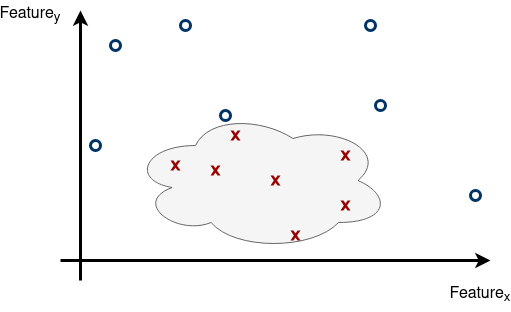
\includegraphics[width=\textwidth]{gfx/AIX-Page-1.drawio.png}
    \vfill
    Proximity $\sim$ similarity
    
    Proximity $\nsim$ same class
\end{frame}

\section{ProtoDash}

\begin{frame}{Overview of ProtoDash}
    \textbf{ProtoDash:}
    \begin{itemize}
        \item For tabular, textual and image data
        \item Model-agnostic
        \item Sample-based explanation
    \end{itemize}

    \vfill
    Accessibility:
    \begin{itemize}
        \item Gurumoorthy et al., ``Efficient data representation by selecting prototypes with importance
weights'', doi: 10.48550/ARXIV.1707.01212., 2017.

        \item \url{https://github.com/Trusted-AI/AIX360}
    \end{itemize}
\end{frame}

\begin{frame}{ProtoDash explaining a prediction}
    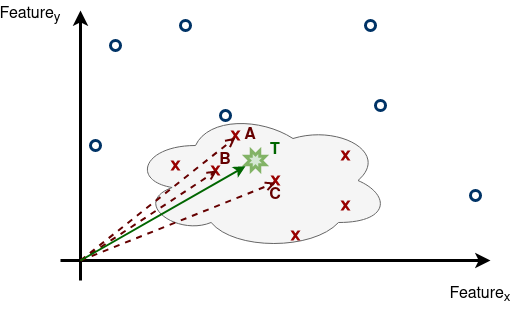
\includegraphics[width=.9\textwidth]{gfx/AIX-Page-2.drawio.png}

    \centering
    \vfill

    \only<1>{
        $\mathbf{t} = ?$
    }
    \only<2>{
        $\mathbf{t} \approx 0.4 \cdot \mathbf{a} + 0.2 \cdot \mathbf{b} + 0.4 \cdot \mathbf{c}$
    }
\end{frame}

\begin{frame}{ProtoDash explaining a dataset}
    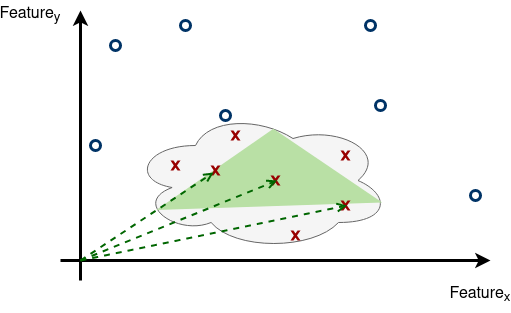
\includegraphics[width=.9\textwidth]{gfx/AIX-Page-3.drawio.png}
    
    Greedy approximation of the class polytope
\end{frame}

\section{LIME}

 \begin{frame}{Motivation of LIME}
     We only have a pre-trained black-box model, without any training data.

     We want to explain a prediction or the model itself.
    \vfill
     \textbf{LIME}:
     \begin{itemize}
        \item Local Interpretable Model-Agnostic Explanations (LIME)
        \item For tabular, textual and image data
        \item Sample-based explanation (for a single prediction), feature-based explanation (for a model explanation)
    \end{itemize}
    \vfill

    Sources:
    \begin{itemize}
        \item MT. Ribeiro, S. Singh, and C. Guestrin, ``Why shoud I trust you?: Explaining the predictions of any classifier'', doi: 10.48550/ARXIV.1602.04938, 2016.
        \item \url{https://github.com/marcotcr/lime}
    \end{itemize}
 \end{frame}

 \begin{frame}{LIME explaining a prediction}
    \only<1>{
        \textbf{Given:} a $\mathbf{z}$ test sample, and an $f$ classifier model
        \vfill
        
        \textbf{Steps of LIME:}
        \begin{enumerate}
            \item generate $\mathcal{Z}'$ new test set by perturbing $\mathbf{z}$
            \item feed $\mathcal{Z}'$ into $f$: $c_i = f(\mathbf{z}_i')$ for each $\mathbf{z}_i' \in \mathcal{Z}'$
            \item weight $(\mathbf{z}_i', c_i)$ pairs by the distance between $\mathbf{z}_i'$ and $\mathbf{z}$
            \item train a simple (e.g. least squares) classifier to separate classes defined by the weighted $(\mathbf{z}_i', c_i)$ pairs
        \end{enumerate}

        \vfill
        \textbf{Local explanation:} the obtained linear model
    }
    \only<2>{
        \centering
        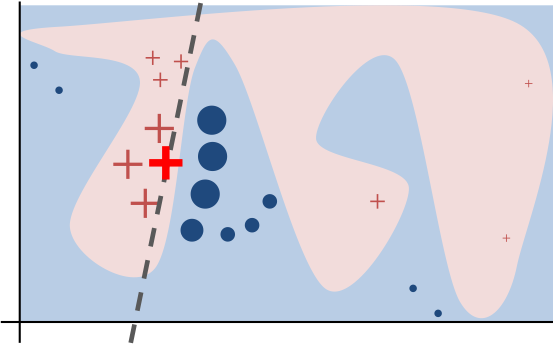
\includegraphics[width=.75\textwidth]{gfx/lime.png}
        
        Red, bold cross is being explained. Classes are shown as background colors, the perturbed samples are shown, and weighed acc. to their distance from the test sample. The local explanation is the dashed line.

        \flushleft
        \vfill
        \footnotesize
        Source: MT. Ribeiro, S. Singh, and C. Guestrin, ``Why shoud I trust you?: Explaining the predictions of any classifier'', doi: 10.48550/ARXIV.1602.04938, 2016.
        \normalfont
    }
 \end{frame}

\begin{frame}{LIME explaining a model}
    \textbf{Goal:} to (globally) explain a black-box classifier

    \vfill
    \textbf{We have:} a local explanation for a single predictions

    \textbf{Idea:}\begin{enumerate}
        \item Let us have local explanations for a variety of test samples
        \item By combining the local explanations, we can achieve an approximation of the global explanation
    \end{enumerate}

    \vfill
    LIME can also do this, and returns an $\mathbf{I}$ vector that explains how different features influences the global predictions.
\end{frame}

\section{Qualitative metrics}

\begin{frame}{ProtoDash}
    \begin{itemize}
        \item Test prediction explanation:
            \begin{itemize}
                \item weights of the returned training samples (comparing training and test samples)
                \item number of returned training samples (How unique is the test sample? Fewer samples $\sim$ more similar test vector)
                \item distance in $\mathbb{R}^d$ of the returned training samples from the test sample (closer vectors $\sim$ more convincing explanation)
            \end{itemize}
        \item Dataset explanation:
            \begin{itemize}
                \item number of prototypical samples (more vectors $\sim$ more difficult distribution)
                \item weights of the prototypical samples (defining the form of the distribution)
            \end{itemize}
    \end{itemize}
\end{frame}

\begin{frame}{LIME}
    \begin{itemize}
        \item Local (test prediction) explanation:
        \begin{itemize}
            \item Coefficients of the features in the Least Squares Estimation (How do the features influence the prediction?)
            \item How much of the test sample has to be changed to receive a different predictions (for image or textual data)? (more to change $\sim$ more well-founded classification)
        \end{itemize}

        \item Global (model) explanation:
        \begin{itemize}
            \item Number of the characterizing features (less feature $\sim$ simpler model; indicating the absence of overfitting). Also to compare black-box models
        \end{itemize}
    \end{itemize}
\end{frame}

\section{Demo}

\sectionNotInTocAndNavigation{Questions?}
%%%%%%%%%%%%%%%%%%%%%%%%%%%%%%%%%%%%%%%%%%%%%%%%%%%
%%%%	toc
%%%%%%%%%%%%%%%%%%%%%%%%%%%%%%%%%%%%%%%%%%%%%%%%%%%
%\begin{frame}
%	\tableofcontents
%\end{frame}


%%%%%%%%%%%%%%%%%%%%%%%%%%%%%%%%%%%%%%%%%%%%%%%%%%%%
%%%%%	introduction
%%%%%%%%%%%%%%%%%%%%%%%%%%%%%%%%%%%%%%%%%%%%%%%%%%%%
%\section{Introduction}
%\begin{frame}[fragile]
%	\frametitle{minflat}
%	The \emph{minflat} theme is a Beamer theme in modern flat design, i.e. emphasising a minimal yet functional design, primarily designed for mathematical talks.\\[.5em]
%
%	You can enable the theme by loading:
%	\begin{verbatim}    \documentclass{beamer}
%    \usetheme{minflat} \end{verbatim}
%    Note that XeTeX and the free Museo Sans 300 font need to be installed. Moreover this theme requires that the following packages are installed:
%	\begin{itemize}
%		\item \emph{tikz}
%		\item \emph{datetime2}
%	\end{itemize}
%\end{frame}
%
%
%\begin{frame}{Design}
%	You can choose between two color schemes. A {\bfseries\color{darkpurple} blue violet} and a {\bfseries\color[RGB]{137,57,94} red purple} variant. Corresponding colours used are green for the {\color{progressbar green} progress bar} (and {\color{beamergreen} examples}) and orange for {\color{beamerorange} alert elements} (cf. \hyperlink{slide::ex-alert-el}{below}).\\[.5em]
%	
%	Sections always start showing an overlay slide containing the section name and a nice progress bar.\\[.5em]
%	
%	All slides have a progress bar on top where the current section is indicated by highlighted green blob and a slightly bolder name.\\[.5em]
%	
%	The date uses the {\fontsize{9pt}{9pt}\selectfont\texttt{datetime2}} package so you can change the format if you wish. You should replace the logo on the title page with our own by setting the appropriate path or just comment out with no harm. At the moment I am a PhD student (Assistant-doctorant) at the University of Luxembourg. 
%\end{frame}
%
%\begin{frame}[fragile]{Theme Options \& Remarks}
%	\begin{center}
%		\arrayrulecolor{darkpurple}
%		\begin{tabular}[]{ll}
%			\toprule
%			{\bfseries Option} 	& {\bfseries Description}\\
%			\midrule
%			purple				& switch to {\bfseries\color[RGB]{137,57,94} red purple} colour scheme\\[0.5em]
%			xcolor={table}		& should be activated to colour tables\\[0.5em]
%			notheorems			& should be activated to use the dummyblock definition\\
%			\bottomrule
%		\end{tabular}
%	\end{center}	
%	Note that if you use the
%	\begin{verbatim}  \usepackage{pgfpages}
%  \setbeameroption{show notes on second screen=right}
%  \setbeamertemplate{note page}[compress] \end{verbatim}
%    to enable notes on the second screen there is a bug in beamer that normal text on frames becomes white. So I added a \texttt{dummyblock} wrapper to solve this issue.
%\end{frame}
%
%
%%%%%%%%%%%%%%%%%%%%%%%%%%%%%%%%%%%%%%%%%%%%%%%%%%%%
%%%%%	Blocks, Alerts \& Math Environments
%%%%%%%%%%%%%%%%%%%%%%%%%%%%%%%%%%%%%%%%%%%%%%%%%%%%
%\section{Blocks, Alerts \& Math Environments}
%\begin{frame}{Blocks, Alerts \& Math Environments}
%	\begin{block}{Notation}
%		This is some notation.
%	\end{block}
%
%	\begin{definition}
%		This is a definition.
%	\end{definition}
%	
%	\begin{remark}
%		And this is a remark.
%	\end{remark}
%\end{frame}
%
%\begin{frame}
%	\begin{theorem}[Existence \& Uniqueness for ...]
%		A theorem is important so it should be emphasised!
%	\end{theorem}
%
%	\begin{proposition}
%		A proposition may be a little less important but it's also worth emphasising!
%	\end{proposition}
%	
%	In the same way we can create lemmata \& corollaries.
%\end{frame}
%
%\begin{frame}\label{slide::ex-alert-el}
%	\begin{example}
%		Examples should be made. Of course normally only the mathematician understands why this text on the blackboard should be an example.
%	\end{example}
%
%	Finally
%		
%	\begin{alertblock}{\includegraphics[width=1cm]{./gfx/mit_logo.png}}
%		An alert block has a catchy colour.
%	\end{alertblock}
%\end{frame}
%
%
%{
%	\definecolor{darkpurple}{RGB}{137,57,94}
%	\definecolor{beamergreen}{RGB}{57,137,100}
%	\definecolor{beamerorange}{RGB}{255,175,0}
%	\begin{frame}{Red purple colour scheme}
%		Finally let us have a look at the second colour scheme:
%		
%		\begin{theorem}[Existence \& Uniqueness for ...]
%			A theorem is important so it should be emphasised!
%		\end{theorem}
%	
%		\begin{example}
%			Examples should be made. Of course normally only the mathematician understands why this text on the blackboard should be an example.
%		\end{example}
%	
%		\begin{alertblock}{Alert, alert}
%			An alert block has a catchy colour.
%		\end{alertblock}
%	\end{frame}
%}
%
%
%%%%%%%%%%%%%%%%%%%%%%%%%%%%%%%%%%%%%%%%%%%%%%%%%%%%
%%%%%	Overlays \& Images
%%%%%%%%%%%%%%%%%%%%%%%%%%%%%%%%%%%%%%%%%%%%%%%%%%%%
%\section{Overlays \& Images}
%\begin{frame}[fragile]
%	\frametitle{Overlays \& Images}
%	Complying with the old saying: \enquote{A picture speaks a thousand words}, we can create frames which only contain a picture by
%	\begin{center}
%		\texttt{\textbackslash imageFrame\{imageURL\}.}
%	\end{center}
%	We can also define an overlay on the left oder right side of the frame. By default the overlay has a width of 150pt. We can adjust as an optional argument.
%	\begin{verbatim} \imageFrameOverlayLeft[optional width]{%
%    ./gfx/horizontallift.pdf}{%
%    Want big impact?}{%
%    Use a big picture.} \end{verbatim}
%\end{frame}
%
%\begin{frame}[fragile]{Test}
%	\begin{center}
%		\begin{tikzpicture}[remember picture, overlay]
%		\blurredimage{0.0, 0.0}{0.1}{./gfx/teszt.jpg}
%		\end{tikzpicture}
%	\end{center}
%	
%	Lehet erre egyébként írni? őúöüóű
%\end{frame}
%
%\begin{frame}[fragile]{Test}
%	\begin{center}
%		\begin{tikzpicture}[remember picture, overlay]
%		\blurredimagesimple{./gfx/test_image.jpeg}{./gfx/blurred_test_image.jpeg}
%		\end{tikzpicture}
%	\end{center}
%	
%	Lehet erre egyébként írni? őúöüóű
%\end{frame}
%
%\begin{frame}{Test2}
%	\blurredframe{./gfx/test_image.jpeg}{./gfx/blurred_test_image.jpeg}
%	Random tartalom kezdődik itt.
%	\vfill
%	És itt végződik.
%\end{frame}
%
%%%%%	image frame with overlay left
%\imageFrameOverlayLeft{%
%./gfx/horizontallift.pdf}{%
%Want big impact?}{%
%Use a big picture.}
%
%%%%%	image frame with overlay right, custom size
%\imageFrameOverlayRight[150pt]{%
%./gfx/horizontallift.pdf}{%
%Need a bigger overlay on the right side?}
%
%
%%%%%%%%%%%%%%%%%%%%%%%%%%%%%%%%%%%%%%%%%%%%%%%%%%%%
%%%%%	Listings, Tables, Highlighted Text \& Tikz
%%%%%%%%%%%%%%%%%%%%%%%%%%%%%%%%%%%%%%%%%%%%%%%%%%%%
%\section{Listings, Tables, Highlighted Text \& Tikz}
%
%\begin{frame}{Listings}
%	\begin{itemize}
%		\item Item $\sharp$1
%		\item Item $\sharp$2
%			\begin{itemize}
%				\item Subitem 2.$\sharp$1
%				\item Subitem 2.$\sharp$2
%			\end{itemize} 
%	\end{itemize}
%	and so on. We can also create highlighted lists:
%	\begin{itemize}[<+- | alert@+>]
%		\item \alert<4>{\only<-3>{Hi!}\only<4>{or here?}}
%		\item you
%		\item there!
%	\end{itemize}
%\end{frame}
%
%\begin{frame}{Tables}
%	\begin{center}
%		\arrayrulecolor{darkpurple}
%		\begin{tabular}[]{lrrl}
%			\toprule
%								& \multicolumn{1}{c}{{\bfseries Dual space}}
%			                    & \multicolumn{1}{c}{{\bfseries Reflexive}}
%			                    & \multicolumn{1}{l}{{\bfseries Norm}} \\
%			\midrule
%			$\mathbb K^n$	& $\mathbb K^n$			& Yes			& $\Vert x\Vert_2 =\left(\sum_{i=1}^n |x_i|^2\right)^{\frac 12}$\\[0.5em]
%			$\ell_p$			& $\ell_q$				& Yes			& $\Vert x\Vert_p = \left( \sum_{i=1}^\infty |x_i|^p \right)^{\frac 1p}$\\[0.5em]
%			$\ell_1$			& $\ell_\infty$			& \alert{No}	& $\Vert x\Vert_1 = \sum_{i=1}^\infty |x_i|$\\[0.5em]
%			$\ell_\infty$	& {\small complicated}	& \alert{No}	& $\Vert x\Vert_\infty = \sup_i |x_i|$\\[0.5em]
%			$L^p(\mu)$		& $L^q(\mu)$			& Yes			& $\Vert f\Vert_p = \left( \int |f|^p \, \mathrm d\mu \right)^{\frac 1p}$\\[0.5em]
%			$L^1(\mu)$		& $L^\infty(\mu)$ 		& \alert{No} 	& $\Vert f\Vert_1 = \int |f| \, \mathrm d\mu$\\
%			\bottomrule
%		\end{tabular}
%	\end{center}
%\end{frame}
%
%%%%%%%%%%%%%%%%%%%%%%%%%%%%%%%%%%%%%%%%%%%%%%%%%%%%
%%%%%	highlighted frame with number and 
%%%%%	optional subtext
%%%%%%%%%%%%%%%%%%%%%%%%%%%%%%%%%%%%%%%%%%%%%%%%%%%%
%\highlightedFrame[such an impressive number should be big!]{89.432.567}
%
%\begin{frame}{Tikz}
%	\begin{center}
%	    \begin{tikzpicture}[scale=.8]
%	        \pgfmathsetseed{2236}
%	
%	        \fill (0,0) circle (2pt);
%		    \draw (0,0) ellipse (5 and 3);
%	    		\node at (5,-2.5) {$D \subsetneq \mathbb R^n$};
%	        
%	        \draw[decorate, decoration={random steps,segment length=5pt,amplitude=10pt}] [darkpurple] plot [smooth, tension=1] coordinates { (0,0) (2,0) (0,2.5) (-3,0) (0,-1.5) (4,1.8)};
%	        \node[darkpurple] at (2.8,-1.5) {BM with $p_t$, $T_t$};
%	        
%	        \node at (5.2,1.8) {$\partial D \ni x_0$};
%	        \fill (4,1.8) circle (1pt);
%	        
%	        \draw[->,beamergreen,thick] (4,1.8) -- (3,1);
%	        
%	        \draw[->,beamerorange,thick] (4,1.8) -- (5,2.6);
%	        \fill (4,1.8) circle (.5pt);
%	    \end{tikzpicture}
%	\end{center}
%	
%	\begin{itemize}
%	    \item Trap, $x_0$ absorbing = Killing Brownian motion = Dirichlet problem
%	    \item {\color{beamergreen} Reflected Brownian motion = Neumann problem}
%	    \item {\color{beamerorange} Wait an go on = Sticky Brownian motion}
%	\end{itemize}
%\end{frame}
%
%%%%%%%%%%%%%%%%%%%%%%%%%%%%%%%%%%%%%%%%%%%%%%%%%%%%
%%%%%	thanks slide, not in toc
%%%%%%%%%%%%%%%%%%%%%%%%%%%%%%%%%%%%%%%%%%%%%%%%%%%%
%\sectionNotInTocAndNavigation{Thank you. Questions?}
%
%
%%%%%%%%%%%%%%%%%%%%%%%%%%%%%%%%%%%%%%%%%%%%%%%%%%%%
%%%%%	conclusion frame
%%%%%%%%%%%%%%%%%%%%%%%%%%%%%%%%%%%%%%%%%%%%%%%%%%%%
%\begin{frame}{Conclusion}
%
%  Let me close addressing some thanks for the inspiration to the \href{https://github.com/matze/mtheme/}{metropolis mtheme}. This theme and its sources \& demo are completely hosted by
%
%  \begin{center}\url{https://github.com/vipowueb/minflat-beamer}\end{center}
%
%  It \emph{itself} is licensed under the
%  \href{http://creativecommons.org/licenses/by-sa/4.0/}{Creative Commons
%  Attribution-ShareAlike 4.0 International License}.
%
%  \begin{center}\ccbysa\end{center}
%\end{frame}

\end{document}